\documentclass[12pt]{article}

\usepackage{graphicx}
\usepackage{color}   %May be necessary if you want to color links
\usepackage{hyperref}
\hypersetup{
    colorlinks=true, %set true if you want colored links
    linktoc=all,     %set to all if you want both sections and subsections linked
    linkcolor=blue,  %choose some color if you want links to stand out
}
\usepackage{floatrow}
\floatsetup[figure]{capposition=bottom}

%verbatim stuff
\usepackage{fancyvrb}


%step enumaration
\usepackage{enumitem}
\newlist{steps}{enumerate}{1}
\setlist[steps, 1]{label = \textbf{Step \arabic*:}}

%page break after sections
\usepackage{titlesec}
\newcommand{\sectionbreak}{\clearpage}

%remove indentation at Paragraph and add line break
\setlength{\parindent}{0em}
\setlength{\parskip}{1em}

\title{MineBike Game Documentation}
\author{Andrew Weller \& [your name here]}
\date{July 2019}

\setcounter{section}{-1}


\begin{document}
\maketitle

\tableofcontents

\section{This Manual}
Hello anonymous developer! Welcome to the MineBike project. If this is not your desired destination you may leave this document now.

This manual is intended to inform the user about the mineBike GAME portion of the code. This manual does not relate to the middleware or the database portion.
If you are looking for documentation on that, you should search elsewhere.

If you are not already aware of what the project is, mineBike is a minecraft mod designed as an alternative to traditional physical therapy for quarantined hospital patients who are unable to go outside to excercise. 

Please refer to the table of contents if you wish to find what you are looking for quickly. Otherwise reading this manual in chronological order should get you up to speed with the game with zero prior knowledge.

\section {Setup}
\begin{steps}
  \item Clone Repository
		\begin{verbatim}
				$ git clone https://github.com/andrewwellercs/mineBikeCopy
		\end{verbatim}

  \item Unzip Forge Source

		Unzip "MinecraftMod/Forge Source/forge-1.7.10-10.13.4.1492-1.7.10-src.zip" into "MinecraftMod/".

		Be sure to overwrite any files.

  \item Run gradle scripts

		Mac/Linux:
	\begin{verbatim}
		$ ./gradlew setupDecompWorkspace --refresh-dependencies
		
		$ ./gradlew eclipse
	\end{verbatim}

	This will create an eclipse workspace in the MinecraftMod/ directory.

  \item 


\end{steps}

\section {Codebase Overview}
\label{sec:overview}
\begin{figure}[h]
	
\includegraphics[scale=0.5]{images/will_smith_with_camera}
	\centering
\end{figure}
The Codebase looks very big, but there are only a few very important parts to it. Most of the code is either not necessary for manipulating the game or is deprecated. Let's take a look at some important packages. 

\subsection{org.ngs.bigx.minecraft.npcs}
\begin{figure}[h]
	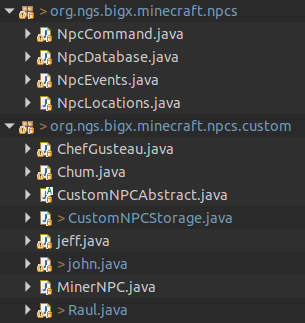
\includegraphics[scale=0.5]{images/tour/orgNgsBigxMinecraftNpcs.png}
	\centering
\end{figure}

This package is largely responsible for the creation of NPCs in the overworld map. Creating npcs in quests is another story and you can learn about it in \hyperref[sec:npcs]{the npcs section}. 

Noteable classes in here include {\bfseries CustomNpcAbstract} which combined with a simple addition to {\bfseries CustomNpcStorage} is a one-stop shop to adding simple npcs into the game. More on that in \hyperref[sec:npcs]{the npcs section}.

\subsection{org.ngs.bigx.minecraft.quests(.custom)}
\begin{figure}[h]
	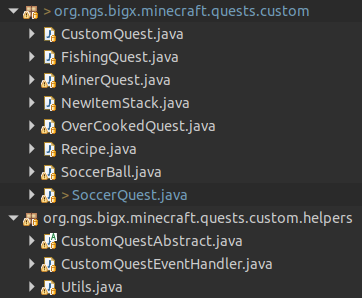
\includegraphics[scale=0.5]{images/tour/orgNgsBigxMinecraftQuestsCustom.png}
	\centering
\end{figure}

This package is responsible for the "quests" or "minigames" that the game has, excluding the original ChasingQuest which was in the game. The questing system is a modular way to build minigames.

\subsection{org.ngs.bigx.minecraft.client.gui.hud}
\begin{figure}[h]
	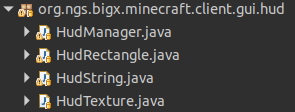
\includegraphics[scale=0.5]{images/tour/orgNgsBigxMinecraftClientGuiHud.png}
	\centering
\end{figure}

This package is very short and specialized. The tools in here can be used to add HUD elements to the game with no knowledge of OpenGL.

More on the usage of this package can be found in the \hyperref[sec:hud]{Hud section}.

\section{Npcs}
\label{sec:npcs}

You might wonder why npcs are first in this guide and not quests. The answer is simple. Npcs are easier to add to the game. So to get your feet wet it is recommended to do this first. Also every quest usually has an npc attached to it. That is the pattern for this game. You start quests by talking to npcs. So once you have created your own npc you can then attach a quest to them and start testing that in the next section.

\subsection{Simple Npcs (overworld)}

Adding Npcs to the overworld is easy.
\begin{figure}[h]
	\caption{A custom NPC made using the CustomNpcAbstract class}
	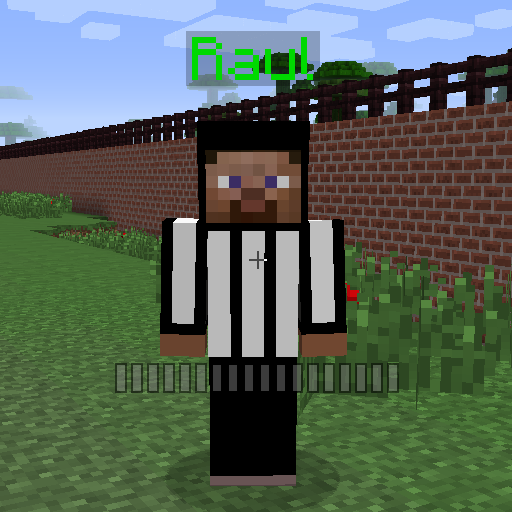
\includegraphics[scale=0.5]{images/npcs/Raul.png}
	\centering
\end{figure}



\subsection{Advanced Npcs (quests/moving)}

\section{Quests}
\label{sec:quests}

\section{Hud}
\label{sec:hud}

\end{document}

